An object moving through a medium displaces mass in the medium it travels through,
A wing moving through the air will displace air particles.
If the total movement of the particles generate a net momentum a force will be generated on the object displacing them, in this case the wing.

The air will thus excert pressure on the wing and it is useful to consider the pressure distribution.
By integrating the pressure distribution over the entire surface of the wing one can find the center of pressure.\cite{aerodynamics}
If the center of pressure and center of gravity are not aligned a torque will also be generated.
The equivalent force and moment can be placed at the center of pressure to simplify calculations.
The aerodynamic force can be split into two parts, one in line with the incoming airflow and one perpendicular to it.
These are usually denoted Lift and Drag forces, see figure \ref{fig:liftdrag} for an illustration of the Lift and Drag forces on an airfoil.

\begin{figure}[h]
    \center
    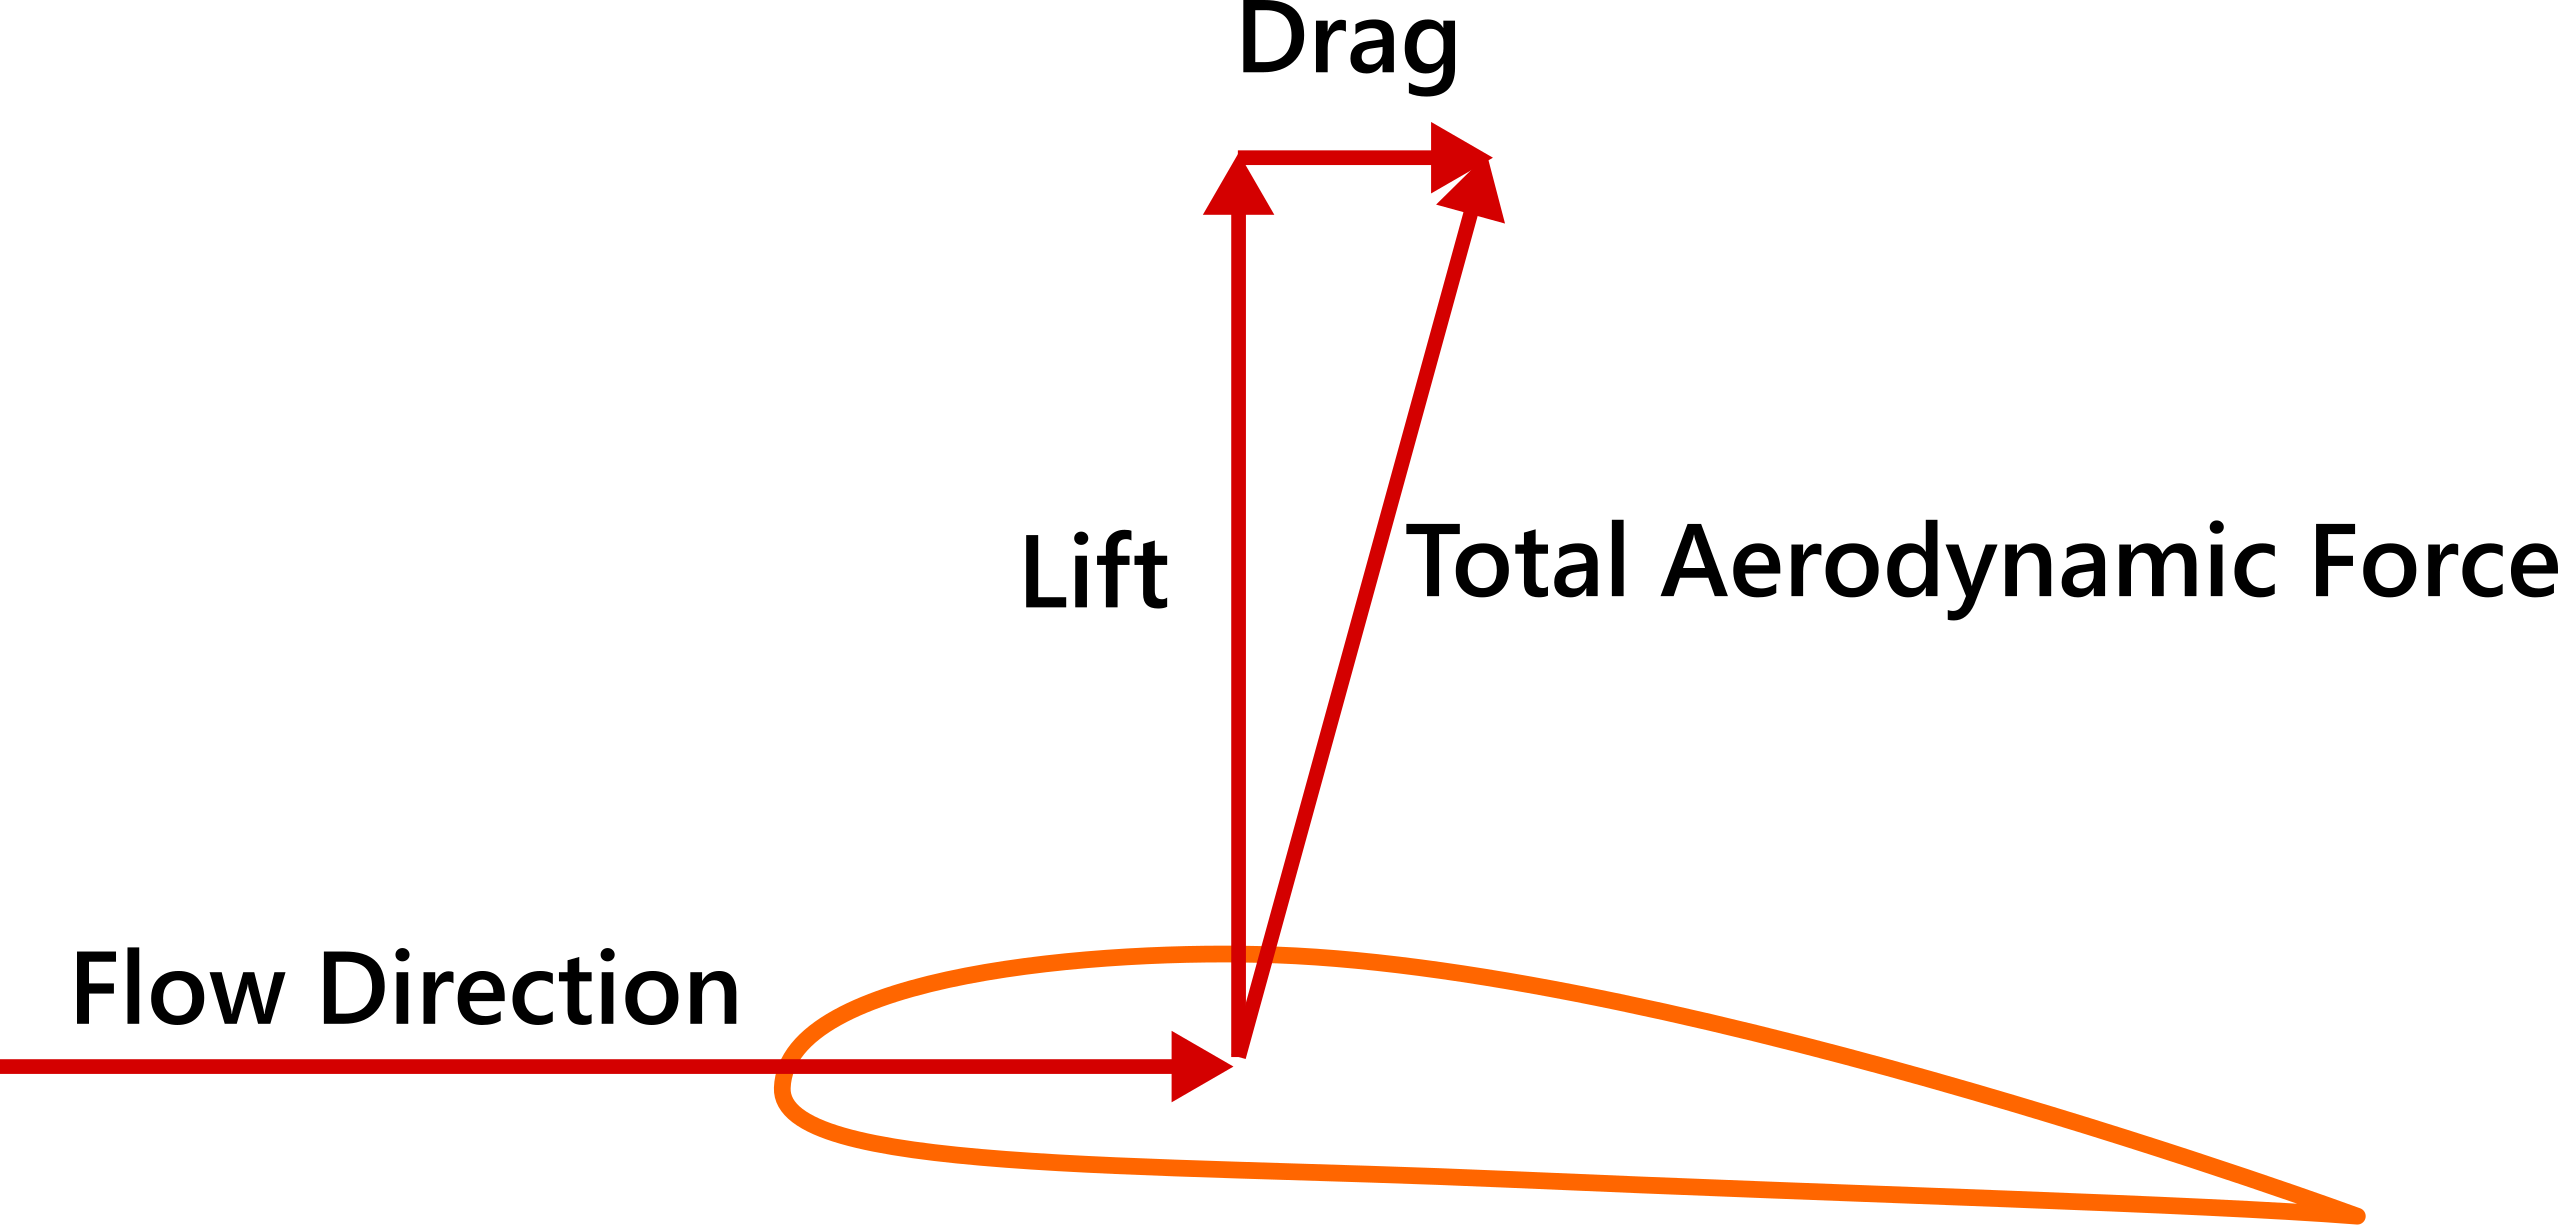
\includegraphics[width=0.4\textwidth]{liftdrag.png}
    \caption{An illustration of how the flow of air over an airfoil generate Lift and Drag. \cite{liftdragpng}}
    \label{fig:liftdrag}
\end{figure}

The lift force can further be broken down into several parts, but aerodynamics is a complicated field, and for the purposes of this thesis we only consider the following:
Lift due to camber (the non symmetry of the wing in the airstream), lift due to angle of attack (the angle which the incoming air makes with the wing) and lift due to control surface deflection.

\subsubsection{Propeller lift}
The force from propellers will be dealt with in greater detail further into this thesis.
But as an introduction they can be thought of as wings moving through the air, only in a rotational matter instead of straight on. 
As they move through the air lift is generated in a similair fashion to normal wings, but since the propeller is mounted at a right angle to the wings the lift force propels the aircraft forward.
The air a propeller displaces is called a wake and will be treated as a separate airflow from the aircraft moving through the air.


%\begin{itemize}
%        \item Bernoulli Equation, center of Pressure, etc
%        \item Basic plate theory
%        \item Aerodynamic center    
%        \item Aerodynamic forces and Moments
%        \begin{itemize}
%            \item Lift, and moment, due to camber
%            \item Lift due to angle of attack
%            \item Drag
%            \item Forces/Moments due to airflow over Ailerons and Elevators
%            \item Forces and Moments due to sideslip and roll
%            \item Forces/Moment due to roll rate, pitch rate and yaw rate
%        \end{itemize}
%        \item Propeller efficiency, airspeed, wake velocity
%    \end{itemize}